% Suha's Proposal
\documentclass{article}


\usepackage{amssymb}
\usepackage{graphicx}
\usepackage{listings}
\usepackage{arydshln}
\usepackage{amsmath}
\usepackage{amsthm}
\usepackage{color}

\usepackage{amsfonts}
\usepackage{xspace}
\usepackage{latexsym}
\usepackage{wasysym} % causing problems with llncs's bold vectors
\usepackage{stmaryrd}
\usepackage{alltt}
\usepackage{mathpartir}
\usepackage[ligature,reserved,inference]{semantic}
\usepackage[lined]{algorithm2e}
\def\ttat{\mtt{@}} % the at package clobbers this
\usepackage{at}
\usepackage{alltt}


%\usepackage[numbers]{natbib}

%\input macros

\newtheorem{dfn}{Definition}
\newtheorem{lem}{Lemma}

\title{Existence of Forward Simulations for Particular Data Structures}
\begin{document}
\maketitle
%!TEX root = draft.tex
\section{Preliminaries}

We formalize several abstraction relations between libraries using a simple
yet universal model of computation, namely labeled transition systems (LTS).
This model captures shared-memory programs with an arbitrary number of threads,
abstracting away the details of any particular programming system irrelevant to
our development.

A \emph{labeled transition system} (LTS) $A=(Q,\Sigma, s_0, \delta)$ over the 
possibly-infinite alphabet $\Sigma$ is a possibly-infinite set $Q$ of states with
initial state $s_0 \in Q$, and a transition relation $\delta \subseteq Q \times @S \times
Q$. The $i$th symbol of a sequence $@t \in @S^*$ is denoted $@t_i$, and the empty
sequence is denoted by $\epsilon$.
An \emph{execution} of $A$ is an alternating sequence of states and transition labels (called also actions)
$\rho = s_0, e_0,s_1\ldots e_{k-1},s_k$ for some $k>0$ such that $\delta(s_i, e_i, s_{i+1})$
for each $i$ such that $0\leq i<k$. We write $s_i\xrightarrow{e_i\ldots e_{j-1}}_A s_j$ as shorthand for 
the subsequence $s_i,e_i,...,s_{j-1},e_{j-1},s_j$ of $\rho$, for any $0\leq i\leq j <k$
(in particular $s_i\xrightarrow{\epsilon}s_i$).
The projection $@t| \Gamma$ of a sequence $@t$ is the maximum subsequence of $@t$ over
 alphabet $\Gamma$. This notation is extended to sets of sequences as usual.
A \emph{trace} of $A$ is the projection $\rho | \Sigma$ of an execution $\rho$ of $A$. 
The set of executions, resp., traces, of an LTS $A$ is denoted by $E(A)$, resp., $Tr(A)$.
An LTS is \emph{deterministic} if for any state $s$ and any sequence $@t\in \Sigma^*$, there is at most
one state $s'$ such that $s\xrightarrow{@t}s'$. More generally, for an alphabet $\Gamma\subseteq \Sigma$,
an LTS is \emph{$\Gamma$-deterministic} if for any state s and any sequence $@t\in \Gamma^*$, there
is at most one state $s'$ such that $s\xrightarrow{@t'}s'$ and $@t$ is a subsequence of $@t'$.

\subsection{Libraries}

Programs interact with libraries by calling named library \emph{methods}, which
receive \emph{parameter values} and yield \emph{return values} upon completion.
We fix arbitrary sets $\<Methods>$ and $\<Vals>$ of method names and
parameter/return values. 

%\begin{example}
%  \label{ex:methods}
%
%  TODO
%
%  The method and value sets for the stack implementation in
%  Figure~\ref{fig:treiber} are $\<Methods> = \set{ \<push>, \<pop> }$ and
%  $\<Vals> = \<Nats> \u \set{ {\tt EMPTY} }$.
%
%\end{example}

\noindent
We fix an arbitrary set $\<Ops>$ of operation identifiers, and for given sets
$\<Methods>$ and $\<Vals>$ of methods and values, we fix the sets
\begin{align*}
  & C = \set{ inv(m,d,k) : m \in \<Methods>, d \in \<Vals>, k \in \<Ops> }
  \text{, and } \\
  & R = \set{ ret(m,d,k) : m \in \<Methods>, d \in \<Vals>, k \in \<Ops> }  
\end{align*}
of \emph{call actions} and \emph{return actions}; each call action $inv(m,d,k)$
combines a method $m \in \<Methods>$ and value $d \in \<Vals>$ with an
\emph{operation identifier} $k \in \<Ops>$. Operation identifiers are used to
pair call and return actions. We denote the operation identifier of a
call/return action $a$ by $\<op>(a)$. Call and return actions $c \in C$ and $r
\in R$ are \emph{matching}, written $c \match r$, when $\<op>(c) = \<op>(r)$. 
We may omit the second field from a call/return action $a$ for methods that have no inputs (e.g., the pop method of a stack) or return values (e.g., the push method of a stack).
A word $\tau \in @S^*$ over alphabet $@S$, such that $(C \u R) \subseteq @S$, is
\emph{well formed} when:
\begin{itemize}

  \item Each return is preceded by a matching call: \\
  $\tau_j \in R$ implies $\tau_i \match \tau_j$ for some $i < j$.

  \item Each operation identifier is used in at most one call/return: \\
  $\<op>(\tau_i) = \<op>(\tau_j)$ and $i < j$ implies $\tau_i \match \tau_j$.

\end{itemize}
We say that the well-formed word $\tau \in @S^*$ is \emph{sequential} when
\begin{itemize}

  \item Operations do not overlap: \\
  $\tau_i, \tau_k \in C$ and $i < k$ implies $\tau_i \match \tau_j$ for some $i < j < k$.

\end{itemize}
Well-formed words represent traces of a library. We assume every set of well-formed
words is closed under isomorphic renaming of operation identifiers. For
notational convenience, we take $\<Ops>=\<Nats>$ for the rest of the paper.
When the value of a certain field in a call/return action is not important we use 
the placeholder $\_$, e.g., $inv(m,\_,k)$ instead of $inv(m,d,k)$ when the input  
$d$ can take any value.

An operation $k$ is called \emph{completed} in a well-formed trace $\tau$ when
$ret(m,d,k)$ occurs in $\tau$, for some $m$ and $d$. Otherwise, it is called \emph{pending}.
%An operation $o$ of an execution $e$ is \emph{completed}
%when both call and return actions $m(u)_o$ and $\<ret>(v)_o$ of $o$ occur in
%$e$, and is otherwise \emph{pending}.

%\begin{example}
%  \label{ex:executions}
%
%  TODO
%
%  The well-formed words
%  \scriptsize
%  \begin{align*}
%     \<push>(0)_1\ \<pop>_2\ \<pop>_3\ \<ret>_1\ \<ret>(0)_3\ \<ret>(0)_2
%    \text{\normalsize, and } 
%    \<push>(0)_1\ \<pop>_2\ \<pop>_3\ \<ret>_1\ \<ret>(0)_2
%  \end{align*}
%  \normalsize
%  represent executions in which one call to the $\<push>(0)$ method overlaps
%  with two calls to $\<pop>$. In the first execution both calls to $\<pop>$
%  have matching return actions $\<ret>(0)$, i.e., the operations $2$ and $3$ are completed,
%  while operation $3$ is pending in the second, it has no matching return.
%
%\end{example}

Libraries dictate the execution of methods between their call and return
points. Accordingly, a library cannot prevent a method from being called,
though it can decide not to return. Furthermore, any library action performed
in the interval between call and return points can also be performed should the
call have been made earlier, and/or the return made later. 
A library thus allows any sequence of
invocations to its methods made by \emph{some} program.

\begin{definition}\label{def:libraries}
A \emph{library} $L$ is an LTS over alphabet $\Sigma$ such that $C \u R\subseteq \Sigma$
and each trace $\tau \in Tr(L)$ is well formed, and
  \begin{itemize}

    \item Call actions $c \in C$ cannot be disabled: \\
    $\tau \cdot \tau' \in Tr(L)$ implies $\tau \cdot c \cdot \tau' \in Tr(L)$
    if $\tau \cdot c \cdot \tau'$ is well formed.
  
    \item Call actions $c \in C$ cannot disable other actions: \\
    $\tau \cdot a \cdot c \cdot \tau' \in Tr(L)$ implies $\tau \cdot c \cdot a \cdot \tau' \in Tr(L)$.
  
    \item Return actions $r \in R$ cannot enable other actions: \\
    $\tau \cdot r \cdot a \cdot \tau' \in Tr(L)$ implies $\tau \cdot a \cdot r \cdot \tau' \in Tr(L)$.
  
  \end{itemize}

\end{definition}

The projection of a library trace over $C\cup R$ is called a \emph{history}. The set of histories of a library $L$ is denoted by $H(L)$.

Note that even a library that implements \emph{atomic methods}, e.g.,~by
guarding method bodies with a global-lock acquisition, admits executions in
which method calls and returns overlap. 
%A library which accesses the client's
%thread identifiers can be modeled by taking thread identifiers as method
%parameters.

%\textcolor{red}{For the below paragraph, I cannot see the equivalence  of informal explanation and formal definition of weakening. I think the formal one should be if a ret comes before a call in $h_1'$ then this order is preserved in $h_2$. But the definition says iff. Ignore this if I am wrong.}
Since libraries only dictate methods’ executions between their respective calls and returns, for any history they admit, they must also 
admit histories with weaker inter-operation ordering, in which calls may happen earlier, and/or returns later. This weakening relation
between histories can be formalized as follows: a history $h_1$ is \emph{weaker} than a history $h_2$, written $h_1 \sqsubseteq h_2$, 
if{f} there exists a well-formed history $h_1'$
obtained from $h_1$ by appending return actions, and deleting call actions,
such that:
\begin{quote}

  $h_2$ is a permutation of $h_1'$ that preserves the order between
  return and call actions, i.e.,~if a given return action occurs before a given
  call action in $h_1'$, then the same holds in $h_2$.

\end{quote}
A call action $inv(\_,\_,k)$ may happen before a return action $ret(\_,\_,k')$ in $h_1$ (the operations $k$ and $k'$ overlapping in time) while it can be permuted after that return action in $h_2$, thus introducing a new inter-operation ordering (operation $k'$ ending before $k$). 

$\overline{H}$ denotes the closure $\set{h: \exists h' \in H.\ h \sqsubseteq h'}$ of a 
history set $H$ under weakening.
A direct consequence of Definition~\ref{def:libraries} is that $H(L)=\overline{H(L)}$ for
every library $L$. A \emph{kernel} of L is any set $K$ such that $\overline{K} = H(L)$.
A library $L$ is called atomic if it has a sequential kernel. 
Atomic libraries are often considered as specifications for concurrent objects. 
In practice, libraries can be made atomic by guarding their methods bodies with global lock acquisitions.

A library $L$ is called a \emph{queue implementation} when its alphabet contains call and return actions defined over $\<Methods>=\{enq,deq\}$ ($enq$ is the name of the methods that enqueue a value, and $deq$ is the name of the methods that dequeue a value) and $\<Vals>=\<Nats>\cup\{{\tt EMPTY}\}$ where {\tt EMPTY} is the value returned by $deq$ when the queue is empty. Similarly, a library $L$ is called a \emph{stack implementation} when $\<Methods>=\{push,pop\}$ and  $\<Vals>=\<Nats>\cup\{{\tt EMPTY}\}$.


%\begin{example}
%  \label{ex:libraries}
%
%  TODO (replace executions with histories)
%
%  Any library which admits the execution
%  \scriptsize
%  \begin{align*}
%    \<push>(0)_1\ \<ret>_1\ \<pop>_2\ \<ret>(0)_2
%  \end{align*}
%  \normalsize
%  with sequential calls to $\<push>$ and $\<pop>$ must also admit
%  \scriptsize
%  \begin{align*}
%    \<push>(0)_1\ \<pop>_2\ \<ret>_1\ \<ret>(0)_2
%    \text{ \normalsize and }
%    \<push>(0)_1\ \<pop>_2\ \<pop>_3\ \<ret>_1\ \<ret>(0)_2
%    \text{\normalsize,}
%  \end{align*}
%  \normalsize
%  among others, yet need not admit an execution
%  \scriptsize
%  \begin{align*}
%    \<push>(0)_1\ \<pop>_2\ \<pop>_3\ \<ret>_1\ \<ret>(0)_3\ \<ret>(0)_2
%  \end{align*}
%  \normalsize
%  with two completed $\<pop>$ operations returning $0$.
%  
%\end{example}




%Systems we consider are labeled transition systems (LTS):
%\begin{dfn}
%An LTS is defined over four-tuples $A=(Q,\Sigma, q_0, \delta)$ where $Q$ is the set of states, $\Sigma$ is the set of transition labels, $q_0 \in Q$ is the initial state and $\delta \subseteq Q \times \Sigma \times Q$ is the transition relation.
%\end{dfn}
%Executions generated by this system are alternating sequence of states and transition labels $\rho = s_0, e_0, s_1,... s_k, e_k,...$ where each $s_i \in Q$, each $e_i \in \Sigma$, $s_0 = q_0$ and each $(s_i, e_i s_{i+1}) \in \delta$. The projection of the sequence $\rho$ over the set $\Pi$ is denoted by $\rho | \Pi$, and it is the maximum subsequence of $\rho$ consisting of elements of $\Pi$. Traces of the LTS are obtained from executions by projecting them over $\Sigma$. For the rest of the paper and in all of the proofs, we consider only finite executions (denoted as $E(A)$) and/or traces (denoted as $Tr(A)$ of the LTSs in focus.

%Libraries are LTSs that provide methods. Let $\mathcal{M}$ be the set of method names and $\mathcal{D}$ be the domain of values as input/output parameters for the methods. Then, this library contains transition labels of the form $inv(m,d,i)$ representing the invocation of method $m \in \mathcal{M}$ with input value $d \in \mathcal{D}$. The third field is the operation identifier for differentiating the different calls of the same method from the set $\mathcal{O}$. For simplicity, we take $\mathcal{O} = \mathbb{N}$ for the rest of the paper. We also assume that methods could have at most one input parameter. If they do not have any input arguments (like pop method of a stack), we can omit the second field from the action. They also provide actions of the form $ret(m,d,i)$ representing the return of method $m \in M$ with value $d \in D$ which has been invoked previously with action $inv(m,d',i)$. Again, we assume that the methods can return at most one parameter and we may omit the second field from the action if they have none (like enqueue method of a queue). Before starting to reason about any set of libraries, we first fix the sets $\mathcal{M}$ and $\mathcal{D}$ and libraries in our focus agree on this sets. For any transition label $e = inv(m,d,i)$ or $e=ret(m,d,i)$, we have the function $oid(e) = i$.
%
%Since libraries are LTSs, they produce traces. A trace $e = e_1, e_2, ..., e_n$ of library $L$ is \emph{well-formed} iff (i) every return matches an earlier invocation: $e_j = ret(m,d,k)$ implies that there exists $i<j$ such that $e_i = inv(m,d',k)$ and (ii) every operation identifier is used at most one invocation/return pair: $oid(e_i) = oid(e_j) = k$ and $i<j$ implies $e_i = inv(m,d,k)$ and $e_j = ret(m,d',k)$. From now on, we assume that libraries produce well-formed traces. Let $f: \mathbb{N} \rightarrow \mathbb(N)$ be a bijection. Then, traces $e$ and $e'$ are equivalent if $e'$ is obtained from $e$ by replacing every action $inv(m,d,k)$ with $inv(m,d,f(k))$ and every action $ret(m,d,k)$ with $ret(m,d,f(k))$. 

\subsection{Refinement and Linearizability}

%\textcolor{red}{A general organizational idea for  this subsection: Linearizability is defined in terms of weakening in which observational actions are just call and return events. Then, we put forward the idea of enriching $\Gamma$ by adding new actions. In the current organization, linearizability is defined after refinement before which this $\Gamma$ extension argument is explained. Hence, people may confuse that notion of linearizability is based on $\Gamma$ set we picked. I propose to first introduce linearizability. Then explain refinement and give Theorem 1.}
Conformance of a library $L_1$ to a specification given as an ``abstract'' library $L_2$ 
is formally captured by \emph{(observational) refinement}. Informally, given two libraries
$L_1$ and $L_2$ implementing the methods of some concurrent object, we
say $L_1$ refines $L_2$ if{f} every computation of every program
using $L_1$ would also be possible were $L_2$ used instead. We assume that a program can 
interact with the library only through call and return actions, and thus refinement can be defined
as history set inclusion. As shown in~\citet{journals/tcs/FilipovicORY10,DBLP:conf/popl/BouajjaniEEH15},
refinement is equivalent to the \emph{linearizability} criterion~\cite{journals/toplas/HerlihyW90} when $L_2$ is an atomic library. 
%We fix a set of methods $\<Methods>$ and values $\<Vals>$.

\textcolor{red}{We have two Definition 1. The problem occurs because we used different commands for definitions.}
\begin{dfn}
Let $L_1$ and $L_2$ be two libraries. 
%agreeing on $\mathcal{M}$ and $\mathcal{D}$ sets. We define the set $A\Sigma = \{inv(m,d,i)| m \in \mathcal{M} \wedge d \in \mathcal{D} \wedge i \in \mathbb{N}\} \cup \{ret(m,d,i)| m \in \mathcal{M}\wedge d \in \mathcal{D} \wedge i \in \mathbb{N}\}$ as abstract transition labels. Note that $A\Sigma \subseteq \Sigma_{L_1}$ and $A\Sigma \subseteq \Sigma_{L_2}$. 
The library $L_1$ \emph{refines} $L_2$ if{f} $H(L_1) \subseteq H(L_2)$.
%We say that $L_1$ \emph{refines} $L_2$ when $H(L_1) \subseteq H(L_2)$.
%for every trace $e \in Tr(L_1)$, there exists a trace $e' \in Tr(L_2)$ such that $e|A\Sigma$ is equivalent to $e'|A\Sigma$.
\end{dfn}

%Linearizability is also a relation between two libraries and it is stricter than refinement. It requires $e'$ in Definition 2 to be a sequential one. A trace $e$ is sequential iff following two conditions hold for its projection to abstract transition labels $e|A\Sigma = e_1, ...e_n$: $(i)$ $e_1 = inv(m,d,k)$ for some $m \in \mathcal{M}, d \in \mathcal{D} and k \in \mathbb{N}$ and $(ii)$ for all $i \in [1,n)$, either $e_i = inv(m,d,k)$ and $e_{i+1} = ret(m,d',k)$ or $e_i = ret(m,d,k)$ and $e_{i+1} = inv(m',d',k')$ for some $m,m' \in \mathcal{M}$, $d,d' \in \mathcal{D}$ and $k,k' \in \mathbb{N}$.

Linearizability~\cite{journals/toplas/HerlihyW90} requires that every history of a concurrent library $L_1$ can be 
``linearized'' to a sequential history admitted by a library $L_2$ used as a specification. 
Formally, a sequential history $h_2$ with only complete operations is called a \emph{linearization} of a history $h_1$ when $h_1 \sqsubseteq h_2$.
A history $h_1$ is \emph{linearizable} w.r.t.~a library $L_2$ if{f} there exists a linearization $h_2$ of $h_1$ such that 
$h_2 \in H(L_2)$. A library $L_1$
is \emph{linearizable} w.r.t. $L_2$, written $L_1 \sqsubseteq L_2$, if{f}
each history $h_1 \in H(L_1)$ is linearizable w.r.t. $L_2$.

\begin{theorem}[\cite{journals/tcs/FilipovicORY10,DBLP:conf/popl/BouajjaniEEH15}]
  $L_1 \sqsubseteq L_2$ if{f} $L_1$ refines $L_2$,
  if $L_2$ is atomic.

\end{theorem}

In the rest of the paper, we discuss methods for proving refinement (and thus, linearizability) focusing mainly on queue and stack implementations.


%!TEX root = draft.tex
\section{Queues With Fixed Dequeue Linearization Points}\label{sec:queues}

The typical abstract implementation of a concurrent queue, denoted by $AbsQ_0$, maintains a sequence of values, the enqueue method adds a value atomically to the beginning of the sequence, and the dequeue method removes a value from the end of the sequence (if any, otherwise it returns ``empty''). In this section, we describe another abstract implementation, denoted as $AbsQ$, which roughly maintains a \emph{partially-ordered set} of values instead of a sequence. We show that there exists a forward simulation from any correct queue implementation where the \emph{dequeue} methods have fixed linearization points (the enqueue methods are unconstrained) to $AbsQ$. This covers all the queue implementations that we are aware of. We describe a forward simulation from the Herlihy\&Wing Queue~\cite{journals/toplas/HerlihyW90} to $AbsQ$.

TODO HOW CAN WE CONVINCE THAT OTHER IMPLEMENTATIONS HAVE THE SAME PROPERTY ?

\subsection{Abstract Queue Implementation}

Before defining the abstract implementation $AbsQ$, we describe a queue implementation listed in Figure~\ref{fig:HerlihyWing} and known as the Herlihy \& Wing Queue~\cite{journals/toplas/HerlihyW90} ($\mathit{HWQ}$ for short), 
where only the dequeue methods have fixed linearization points. 

\begin{wrapfigure}{l}{5.7cm}
\vspace{-8mm}
\begin{lstlisting}
void enq(int x){
  i = back++;
  items[i] = x;
}
int deq() {
  while (1) {
    range = back - 1;
    for (int i = 0; i <= range; i++){
      x = swap(items[i],null);
      if ( x != null ) return x;
    }
  }
}
  \end{lstlisting}
\vspace{-5mm}
\caption{Herlihy \& Wing Queue. We assume that every statement is atomic.}
\label{fig:HerlihyWing}
\vspace{-6mm}
\end{wrapfigure}
The shared state consists of an array {\tt items} storing the values in the queue and a counter {\tt back} storing the index of the first unused position in {\tt items}. Initially, all the positions in the array are {\tt null} and {\tt back} is 0.
An enqueue method starts by reserving a position in {\tt items} ({\tt i} stores the index of this position and {\tt back} is incremented so the same position can't be used by other enqueue operations) and then, stores the input value {\tt x} at this position. The dequeue method traverses the array {\tt items} starting from the beginning and atomically swaps {\tt null} with the encountered value. If the value is not {\tt null}, then the dequeue returns that value. If it reaches the end of the array, then it restarts.

The linearization points of the enqueue methods are not fixed, they depend on dequeue operations executing in the future. Consider the following trace with two concurrent enqueues (${\tt i}(k)$ represents the value of {\tt i} in operation $k$):
\begin{align*}
inv(enq,x,1)\ \ \ inv(enq,y,2)\ \ \ {\tt i}(1) = \mbox{{\tt bck++}}\ \ \ {\tt i}(2) = \mbox{{\tt bck++}}\ \ \ {\tt items[i(2)]} = y
\end{align*}
%\begin{align*}
%inv(enq,x,1)\ inv(enq,y,2)\ ({\tt i}_1 = 0,{\tt bck} = 1)\ ({\tt i}_2 = 1,{\tt bck} = 2)\ ({\tt items[1]} = y)
%\end{align*}
Assuming that the linearization point corresponds to the assignment of {\tt i}, the history of this trace should be linearized to $inv(enq,x,1)\ ret(enq,1)\ inv(enq,y,2)\ ret(enq,2)$. However, a dequeue operation executing until completion after this trace will return value $y$ (only position $1$ is filled in the array {\tt items}) which is not consistent with this linearization. On the other hand, assuming that enqueues should be linearized at the assignment of {\tt items[i]} and extending the trace with ${\tt items[i(1)]} = x$ and a completed dequeue that in this case returns $x$, leads to the following incorrect linearization:
\begin{align*}
inv(enq,y,2)\ ret(enq,2) inv(enq,x,1)\ ret(enq,1)\ inv(deq,3)\ ret(deq,1,3).
\end{align*}

The dequeue method has a fixed linearization point which corresponds to an execution of {\tt swap} returning a non-null value. This action alone contributes to the effect of that value being removed from the queue. This claim will be formally proved in Section~\ref{ssec:HerlihyWing}.

Since the linearization points of the enqueues are not fixed, it is not possible to define a forward simulation from $\mathit{HWQ}$ to the standard abstract implementation $AbsQ_0$. In the following, we describe the abstract implementation $AbsQ$ for which such a forward simulation does exist.

Informally, $AbsQ$ records the happens-before order between enqueue operations for which the added value has not been removed by a dequeue operation. The linearization point of a dequeue operation with return value $d\neq{\tt EMPTY}$ is enabled only if the happens-before order stored in the current state contains a minimal enqueue operation that adds the value $d$. The effect of the linearization point is that the minimal enqueue is removed from the current state and the return value is recorded in the library state. When the return value is {\tt EMPTY}, the linearization point of a dequeue is enabled only if the current state stores only pending enqueue operations (the dequeue overlaps with all the enqueue operations stored in the current state and it can be linearized before all of them).  
The return of a dequeue is enabled only if the returned value matches the one fixed at the linearization point. 
%\textcolor{red}{Important: I think EMPTY return is problematic and I defined it wrong in my machine too. We should be able to return EMPTY if there are only pending nodes. Consider the following history of $AbsQ_0$: $inv(enq, d_1,k_1), inv(enq, d_2,k_2), inv(deq, k_3), lin(deq, \texttt{EMPTY}, k_3)$. This history should be reflected in $AbsQ$ by enabling lin \texttt{EMPTY} of dequeue when there are pending nodes. We also need to update the rules in figure.}

\begin{wrapfigure}{l}{7cm}
\vspace{-8mm}
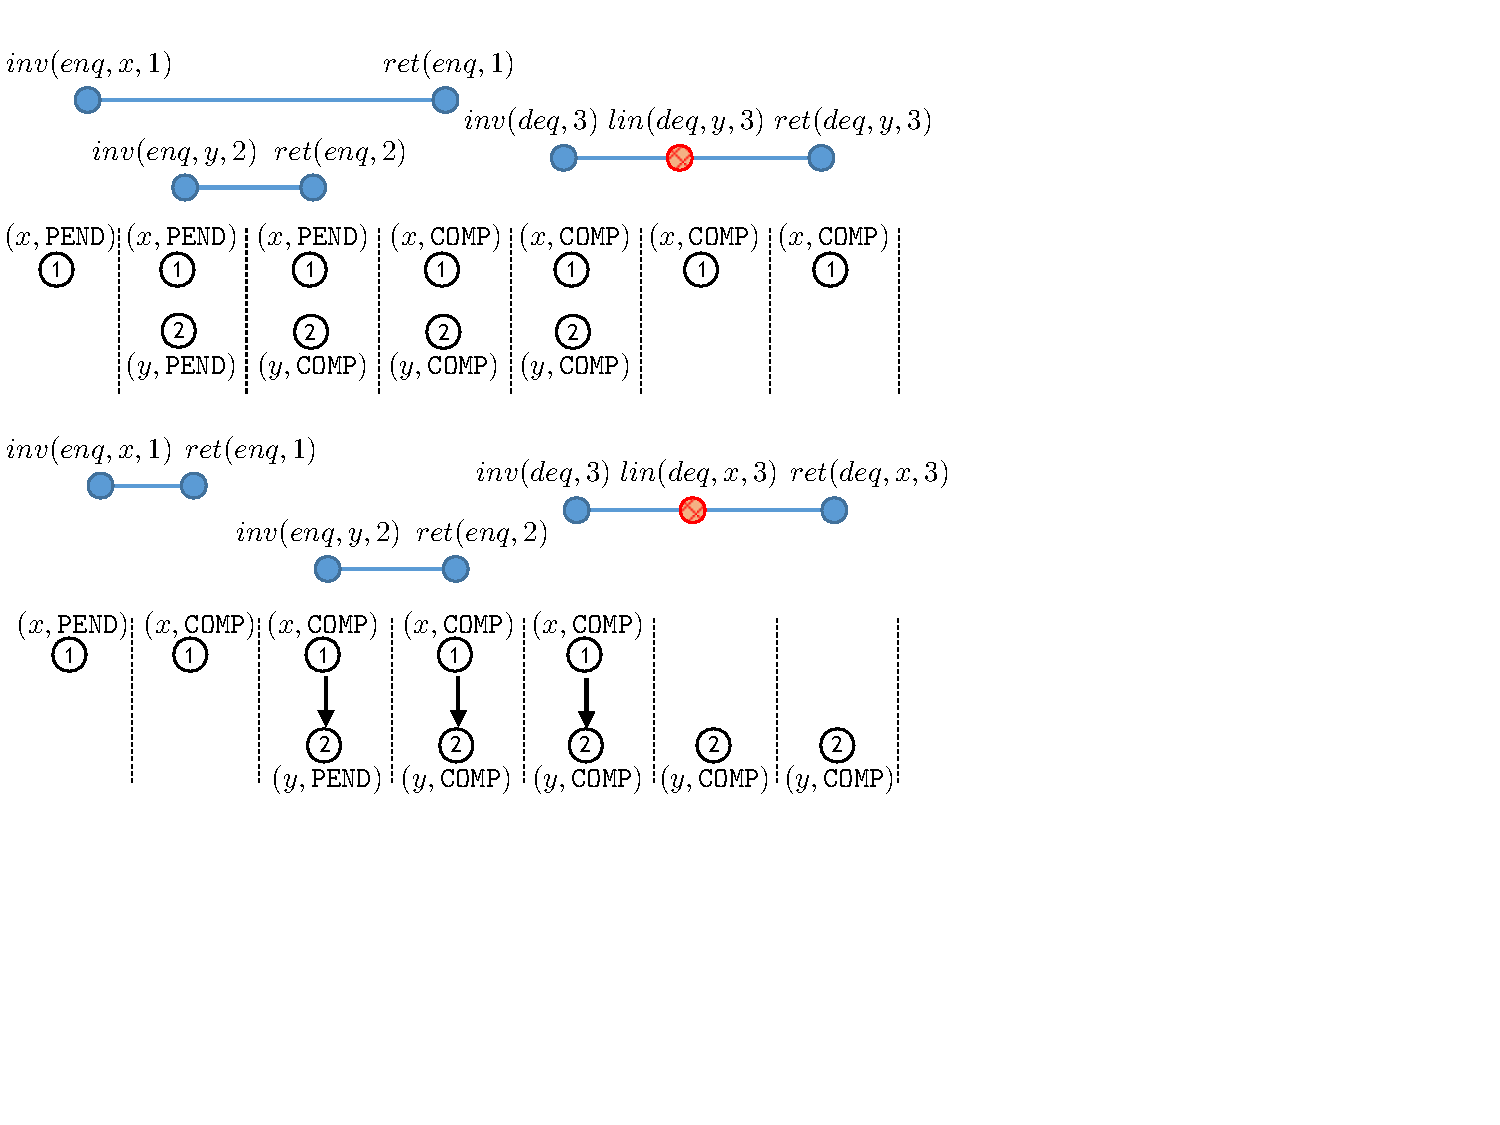
\includegraphics[width=7cm]{fig-queue12.pdf}
%
%\vspace{2mm}
%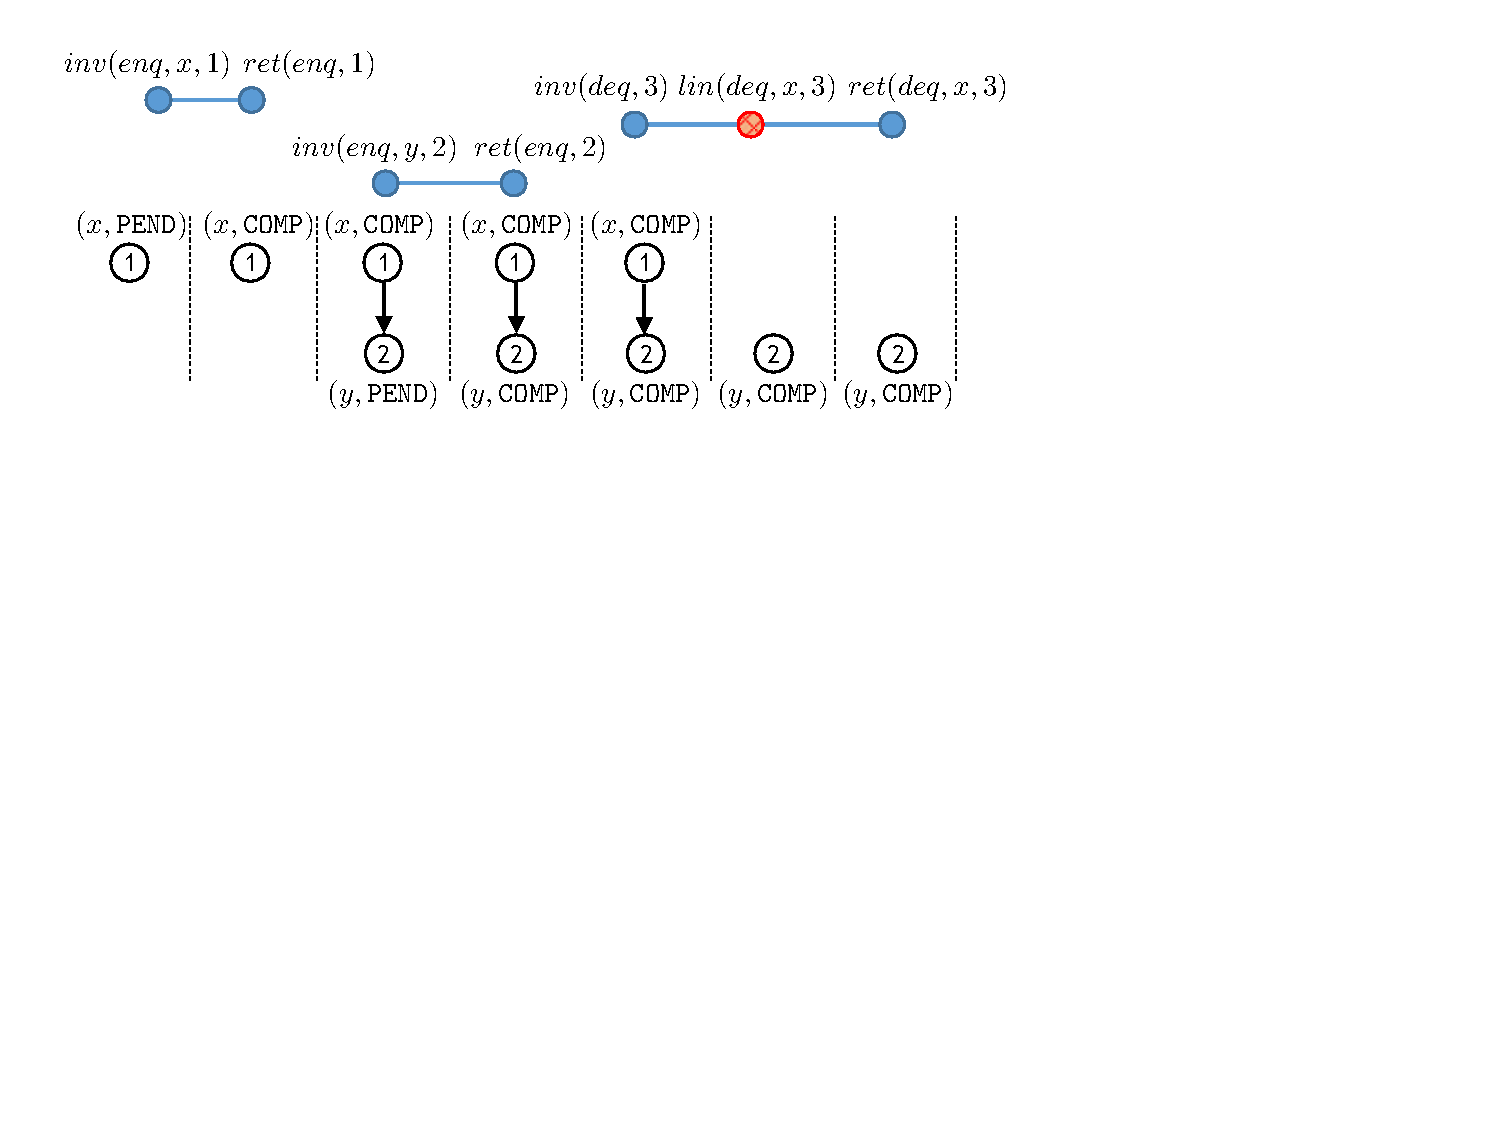
\includegraphics[width=7cm]{fig-queue2.pdf}
\vspace{-5mm}
\caption{Simulating queue histories with $AbsQ$. The order between actions is from left to right.}
\label{fig:queueSim}
\vspace{-10mm}
\end{wrapfigure}
Figure~\ref{fig:queueSim} pictures two executions of $AbsQ$ for two extended histories (that include dequeue linearization points). The state of $AbsQ$ after each action is pictured as a graph below the action. The nodes of this graph represent enqueue operations and the edges happens-before constraints. Each node is labeled by a value (the input of the enqueue) and a flag {\tt PEND} or {\tt COMP} showing whether the operation is pending or completed. For instance, in the case of the first history, the dequeue linearization point $lin(deq,y,3)$ is enabled because the current happens-before contains a \emph{minimal} enqueue operation with input $y$. Note that a linearization point $lin(deq,x,3)$ is also enabled at this state.

Formally, the states of $AbsQ$ are tuples $\tup{O,<,\ell,rv,cp}$ where $O\subseteq \<Ops>$ represents a set of operation identifiers (of previously invoked enqueue operations), $<\subseteq O\times O$ is a strict partial order, $\ell: O -> \<Vals>\times\{\tt{PEND,\tt{COMP}}\}$ labels every identifier with a value and a flag that records whether the operation is pending or completed (this flag is used to track the happens-before order), $rv:\<Ops> ~> \<Vals>$ records the return value of a pending dequeue fixed at its linearization point ($~>$ denotes a partial function), and $cp:\<Ops> ~> \{A_1,A_2,R_1,R_2,R_3\}$ records the control point of every enqueue ($A_1, A_2$) or dequeue ($R_1,R_2,R_3$) operation.
The initial state has all these components set to $\emptyset$ and the transition relation $->$ is defined in Fig.~\ref{fig:transitions:AbsQ}. The alphabet of $AbsQ$ contains call/return actions and dequeue linearization points. The latter are denoted by $lin(deq,d,k)$ where $d\in \<Vals>$, $k\in\<Ops>$. $Lin(deq)$ is the set of all such actions.

Concerning enqueue operations, the rule {\sc call-enq} orders the invoked operation after all the completed enqueue operations stored in the current state, and the rules {\sc ret-enq1}/{\sc ret-enq2} flip the corresponding flag from {\tt PEND} to {\tt COMP} provided that the operation is still present in the current state. For dequeue operations, {\sc call-deq} has no effect other than incrementing the control point and {\sc ret-deq} checks whether the return value is the same as the one fixed at the linearization point. The linearization point rule {\sc lin-deq1} corresponds to the case of a non-empty queue, showing that $lin(deq,d,k)$ is enabled only if the value $d$ has been added by an enqueue which is minimal in the current happens-before order. When it is enabled, it removes the enqueue adding $d$ from the state. The linearization point rule {\sc lin-deq2} corresponds to the case of dequeue operations linearized with an {\tt EMPTY} return value.

\begin{figure} [t]
{\scriptsize
  \centering
  \begin{mathpar}
    \inferrule[call-enq]{
      k\not\in dom(cp) \\ 
      d\neq {\tt EMPTY}
    }{
      O,<,\ell,rv,cp
      \xrightarrow{inv(enq,d,k)}
      %O\cup\{k\},<\cup \{(k',k): \ell_2(k')={\tt COMP}\},\ell[k\mapsto (d,{\tt PEND})],rv,cp[k\mapsto 1]
      O\cup\{k\},<\cup\ {\tt COMP}(O)\times\{k\},\ell[k\mapsto (d,{\tt PEND})],rv,cp[k\mapsto A_1]
    }\hspace{5mm}

    \inferrule[call-deq]{
      k\not\in dom(cp) \\ 
    }{
      O,<,\ell,rv,cp
      \xrightarrow{inv(deq,k)}
      O,<,\ell,rv,cp[k\mapsto R_1]
    }\hspace{5mm}
    \inferrule[ret-deq]{
       cp(k) = R_2 \\
       rv(k)=d  
    }{
      O,<,\ell,rv,cp
      \xrightarrow{ret(deq,d,k)}
      O,<,\ell,rv,cp[k\mapsto R_3]
    }\hspace{5mm}

    \inferrule[ret-enq1]{
      cp(k) = A_1 \\
      k \in O \\
      \ell(k) = (d,{\tt PEND}) 
    }{
      O,<,\ell,rv,cp
      \xrightarrow{ret(enq,k)}
      O,<,\ell[k\mapsto (d,{\tt COMP})],rv,cp[k\mapsto A_2]
    }\hspace{5mm}
    \inferrule[ret-enq2]{
      cp(k) = A_1 \\
      k \not\in O 
    }{
      O,<,\ell,rv,cp
      \xrightarrow{ret(enq,k)}
      O,<,\ell,rv,cp[k\mapsto A_2]
    }\hspace{5mm}

    \inferrule[lin-deq1]{
       cp(k) = R_1 \\
       d\neq{\tt EMPTY} \\
       k'\in min(O) \\ 
       \ell_1(k')=d
    }{
      O,<,\ell,rv,cp
      \xrightarrow{lin(deq,d,k)}
      O\setminus \{k'\},<\uparrow k',\ell,rv[k\mapsto d],cp[k\mapsto R_2]
    }\hspace{5mm}
    \inferrule[lin-deq2]{
       cp(k) = R_1 \\
       \forall o\in O. \ell_2(o)={\tt EMPTY}
    }{
      O,<,\ell,rv,cp
      \xrightarrow{lin(deq,{\tt EMPTY},k)}
      O,<,\ell,rv[k\mapsto {\tt EMPTY}],cp[k\mapsto R_2]
    }\hspace{5mm}    
      \end{mathpar}
  }
 \vspace{-5mm}
  \caption{The transition relation of $AbsQ$. We use the following notations: $\ell_i(k)$ denotes the projection of $\ell(k)$ over the $i$-th component, for each $i\in\{1,2\}$, ${\tt COMP}(O)=\{k\in O: \ell_2(k)={\tt COMP}\}$, $\mathit{f}[x\mapsto y]$ is the function $g$ such that $g(z)=f(z)$ for all $z\neq x$ in the domain of $f$, and $g(x)=y$, $min(O)$ is the set of elements of $O$ which are minimal in the order relation $<$, and $<\uparrow k$ denotes the relation $<$ where all the pairs containing $k$ have been removed.
  %\textcolor{red}{Call-Enq must have $d!= \texttt{EMPTY}$ as a premise. Also lin deq returning empty must be changed as before.}
  }
  \label{fig:transitions:AbsQ}
\vspace{-6mm}
\end{figure}

Both methods have a fixed linearization point when the update of the shared sequence happens. Let $AbsQ_0$ denote this implementation~\footnote{For $\<Methods>=\{enq,deq\}$, the alphabet of $AbsQ_0$ is $C\cup R\cup Lin$.} (formally defined in Appendix~\ref{app:absImplQueue}).
The following result states that the library $AbsQ$ has exactly the same set of histories as the standard abstract library $AbsQ_0$ (see Appendix~\ref{app:absImplQueue} for a proof).

\begin{theorem}\label{th:absImplQueue}
$AbsQ$ is a refinement of $AbsQ_0$ and vice-versa.
\end{theorem}

A trace of a queue implementation is called \emph{$Lin(deq)$-complete} when every completed dequeue has a linearization point, i.e., TODO. A queue implementation $L$ over alphabet $\Sigma$ is called \emph{with fixed dequeue linearization points} if{f} $C\cup R\cup Lin(deq)\subseteq \Sigma$ 
and every trace $@t\in Tr(L)$ is $Lin(deq)$-complete.

TODO NEEDS DATA INDEPENDENCE FOR THE LINEARIZATION POINT TRANSITIONS TO BE DETERMINISTIC

The following result shows that $C\cup R\cup Lin(deq)$-forward simulations are a sound and complete proof method for showing the correctness of a queue implementation with fixed dequeue linearization points (up to the correctness of the linearization points). It is obtained from Theorem~\ref{th:absImplQueue} and Theorem~\ref{th:forSim} using the fact that the alphabet of $AbsQ$ is exactly $C\cup R\cup Lin(deq)$ and $AbsQ$ is deterministic.

\begin{corollary}
A queue implementation $L$ with fixed dequeue linearization points is a $C\cup R\cup Lin(deq)$-refinement of $AbsQ_0$ if{f} there exists a $C\cup R\cup Lin(deq)$-forward simulation from $L$ to $AbsQ$.
\end{corollary}

\subsection{A Correctness Proof For Herlihy\&Wing Queue}\label{ssec:HerlihyWing}

We describe a forward simulation $\mathit{fs}$ from $\mathit{HWQ}$ to $AbsQ$. Essentially, an $AbsQ$ state associated by $\mathit{fs}$ to a $\mathit{HWQ}$ state consists of all the  enqueue operations for which the input is still present in the array {\tt items} and all the pending enqueue operations that have at most reserved an array position, ordered by a relation $<$ satisfying the following: 
\begin{itemize}
	\item[(a)] pending enqueues are maximal, i.e., for every two enqueues $k$ and $k'$ such that $k'$ is pending, we have that $k'\not< k$,
	\item[(b)] $<$ is consistent with the order in which positions of {\tt items} have been reserved, i.e., for every two enqueues $k$ and $k'$ such that ${\tt i}(k) < {\tt i}(k')$, we have that $k' \not< k$,
	\item[(c)] an enqueue which has reserved an array position $i$ %and executed only the first statement 
	can't be ordered before another enqueue that has reserved a position $j \geq i$ when the position $i$ has been ``observed'' by a non-linearized dequeue that may ``observe'' $j$ in the current array traversal, i.e., for every two enqueues $k$ and $k'$, and a dequeue $k_d$, such that 
	
	\noindent
	{\small
	\begin{align}
	\hspace{-8mm}
	{\tt x}(k_d)={\tt null} \land {\tt i}(k') \leq {\tt range}(k_d) \land {\tt i}(k) \leq {\tt i}(k_d) \leq {\tt i}(k')
	 \land ({\tt i}(k) = {\tt i}(k_d) => k_d\atCP {\tt if}\text{-}{\tt inc}) \label{eq:inst}
	\end{align}}
	
	\noindent
	we have that $k \not< k'$. The predicate $k_d\atCP {\tt if}\text{-}{\tt inc}$ holds when the dequeue $k_d$ is at a control point after a {\tt swap} returning {\tt null} and before the increment of {\tt i}.
\end{itemize}

An enqueue is labeled by $(d,{\tt PEND})$ where $d$ is the input value if it's pending and by  $(d,{\tt COMP})$, otherwise. Also, for every dequeue operation $k$ such that ${\tt x}(k)=d\neq {\tt null}$, we have that $rv(k)=d$.

We show that $\mathit{fs}$ is indeed a $C\cup R\cup Lin(deq)$-forward simulation. Let $s$ and $t$ be states of $\mathit{HWQ}$ and $AbsQ$, respectively, such that $(s,t)\in\mathit{fs}$. 
We omit discussing the trivial case of transitions labeled by call and return actions which are simulated by similar transitions of $AbsQ$ (for the return a dequeue operation $k$, we use the equality between the local variable ${\tt x}(k)$ in $s$ and the component $rv(k)$ in $t$). 
%\textcolor{red}{ I think it is good to mention again that call/return actions in HWQ correspond to the same call/return actions in AbsQ (without any other internal action). I also think that invoke enqueue operation is non-trivial. Preservation of the strict partial order and all of the above items a, b and c needs to be rechecked.}

We show that each internal step of an enqueue or dequeue, except the execution of {\tt swap} returning a non-null value in dequeue (which represents its linearization point), is simulated by an \emph{empty} sequence of $AbsQ$ transitions, i.e., for every state $s'$ obtained through one of these steps, if $(s,t)\in\mathit{fs}$, then $(s',t)\in\mathit{fs}$ for each $AbsQ$ state $t$. We focus on the following essential property, called \emph{monotonicity}: the set of possible orders $<$ associated by $\mathit{fs}$ to $s'$ doesn't exclude any order $<$ associated to $s$.
%Essentially, this boils down to showing that the constraints over $<$ in the definition of $\mathit{fs}$ are an invariant for these steps.

Concerning enqueues, let $s'$ be the state obtained from $s$ when a pending enqueue $k$ reserves an array position. This enqueue operation must be maximal in both $t$ and any state $t'$ related to $s'$ (because it is pending). Moreover, there is no dequeue that can ``observe'' this position before restarting the array traversal. Therefore, item (c) in the definition of $<$ doesn't constrain the order between $k$ and some other enqueue neither in $s$ nor in $s'$. Since this transition doesn't affect the constraints on the order between enqueue operations different from $k$ (their local variables remain unchanged), we have that monotonicity holds. This property is trivially satisfied by the second step of enqueue which doesn't affect {\tt i}.

To prove monotonicity in the case of dequeue internal steps different from its linearization point, it is important to track the non-trivial instantiations of item (c) in the definition of $<$ over the two states $s$ and $s'$., i.e., the triples $(k,k',k_d)$ for which (\ref{eq:inst}) holds. Instantiations that are enabled only in $s'$ may in principle lead to a violation of monotonicity (since they restrict the orders $<$ associated to $s'$). For the two steps that begin an array traversal, i.e., reading the index of the last used position and setting the iterator {\tt i} to $0$, there exist no  such new instantiations in $s'$ because the value of {\tt i} is either not set or $0$. % (it is trivial to notice that applying these steps doesn't disable such instantiations that were possible in $s$). 
%The same holds for the step incrementing the iterator {\tt i}. 
%
%The execution of {\tt swap} returning {\tt null} may introduce one new non-trivial instantiation $(k,k',k_d)$ of item (c).
%We write ${\tt i}_s(k)$ to refer to the value of the variable {\tt i} of operation $k$ in state $s$. Assume that indeed, there exist two enqueue operations $k$ and $k'$ such that ${\tt i}_{s'}(k) < {\tt i}_{s'}(k_d) \leq {\tt i}_{s'}(k')$, ${\tt x}_{s'}(k_d)={\tt null}$, ${\tt i}_{s'}(k') \leq {\tt range}_{s'}(k_d)$ TODO SWAP. Since {\tt swap} returnes {\tt null}, the position ${\tt i}_{s'}(k_d)$
%
%
% and ${\tt i}_{s}(k) = {\tt i}_{s'}(k_d)$. The latter constraint guarantees that this instantiation is not enabled in state $s$. The increment of {\tt i} being enabled, implies that 
%
The same is true for the increment of the iterator {\tt i} in a dequeue $k_d$ since the predicate $k_d\atCP {\tt if}\text{-}{\tt inc}$ holds in state $s$.
The execution of {\tt swap} returning {\tt null} in a dequeue $k_d$ enables new instantiations $(k,k',k_d)$ in $s'$, thus adding potentially new constraints $k\not< k'$. We show however that these instantiations are vacuous because $k$ must be a pending enqueue in $s$ and thus maximal in any order relation $<$ associated by $\mathit{fs}$ to $s$.
Let $k$ and $k'$ be two enqueue operations such that together with the dequeue $k_d$ they satisfy the property (\ref{eq:inst}) in $s'$ but not in $s$. 
We write ${\tt i}_s(k)$ to refer to the value of the variable {\tt i} of operation $k$ in state $s$. 
This implies that ${\tt i}_{s'}(k) = {\tt i}_{s'}(k_d) \leq {\tt i}_{s'}(k')$ and ${\tt items}[{\tt i}_{s'}(k_d)]={\tt null}$. The latter implies that the enqueue $k$ didn't executed
the second statement and it is pending (because the position it reserved is still {\tt null}). Finally, checking whether the value returned by {\tt swap} is {\tt null} doesn't modify any of the variables in property  (\ref{eq:inst}) and also, it doesn't change the valuation of the predicate $\atCP {\tt if}\text{-}{\tt inc}$.

Finally, we show that the linearization point of a dequeue $k$ of $\mathit{HWQ}$, i.e., an execution of {\tt swap} returning a non-null value $d$, from state $s$ and leading to a state $s'$ is simulated by a transition labeled by $lin(deq,d,k)$ of $AbsQ$ from state $t$. By the definition of $\mathit{HWQ}$, there exists a unique enqueue $k_e$ which filled the position updated by $k$, i.e., ${\tt i}_s(k_e)=i_s(k)$ and ${\tt x}_{s'}(k)={\tt x}_s(k_e)$. We show that $k_e$ is minimal in the order relation $<$ of $t$ which implies that $lin(deq,d,k)$ is enabled in $t$. Thus, instantiating item (c) in the definition of $<$ with $k'=k_e$ and $k_d=k$ we get that every enqueue that reserved a position smaller than the one of $k_e$ can't be ordered before $k_e$ in the order $<$. Also, applying item (b) with $k=k_e$ we get the same for every enqueue that reserved a bigger position. An enqueue that didn't reserved a position is by definition maximal in the order $<$ and therefore, not a predecessor of $k_e$. The state $t'$ obtained from $t$ through a $lin(deq,d,k)$ transition is related to $s'$ because essentially, (1) the value added by $k_e$ is not anymore present in {\tt items} which implies that $k_e$ doesn't occur in any $AbsQ$ state related to $s'$, and (2) the value of ${\tt x}(k)$ is set to $d\neq {\tt null}$ which implies that $rv(k)$ is set to $d$ in every $AbsQ$ state related to $s'$.


\section{Existence of Forward Simulations for Stack Implementations that have Fixed Pop Linearization Points}
\section{Relaxation for the Data Structures Without Fixed Remove Linearization Points}
We have observed that some implementations (like time-stamped stack) do not have fixed remove (pop) linearization points that will correspond to $lin(pop,e,k)$ where $e$ could be a data value or $\texttt{EMPTY}$. However, we observe that, these implementations contain some points in their pop methods that logically removes the element from the pool. We call them commit points. If a method of a library has a fixed linearization  point, it is also a commit point. In this sense, commit points are weaker versions of fixed linearization points. Fixed linearization point of a pop preserves the following properties:
\begin{itemize}
\item If a $ret$ comes before a linearization point in the concrete execution, this order is preserved in the linearization of this execution.
\item If a $lin$ pop comes before another $lin$ pop in the concrete execution, this order is preserved in the linearization of this execution.
\item If a $lin$ pop comes before an $inv$ in the concrete execution, this order is preserved in the linearization of this execution. 
\end{itemize} 
A commit point is weaker than a fixed linearization point in the sense that it does not need to satisfy the first and the second conditions. 

To our intuition, if a pop (remove) method has multiple finite linearization points, commit point is the latest element in this set. We have never observed an implementation in which a pop is linearized after it logically removes the element from the data structure. 

From now on, we will restrict ourselves to stacks, since our example implementation that we will show linearizability of is the time-stamped (TS) stack. However, the notions and the machines we will introduce can be extended to queues easily. 

We fix $\mathcal{M} = \{push, pop\}$ and $\mathcal{D} = \mathbb{N} \cup \{\texttt{EMPTY}\}$. We extend the alphabet $A\Sigma$ for stacks with commit points as $ACS\Sigma = A\Sigma \cup \{com(pop,d,k)|d \in \mathcal{D}, k \in \mathcal{M}\}$. We define cs-refinement and cs-linearizability as we defined q-refinement, q-linearizability in the previous sections. We also change definitions of backward and forward simulation relations for stacks with commit points as we do in the previous sections by replacing linearization points with commit points in this extensions. Lemma 1 of the first section still holds with new simulation relation definitions and cs-linearizability and cs-linearizability implies the original linearizability definition. 

Our road map for this section is as follows: We will first introduce an intermediate stack machine $L_I$ that will be deterministic with respect to the alphabet $ACS\Sigma$. We will show that $L_I$ is equivalent to the standard abstract stack $L_A$ defined in the previous section with respect to the language $A\Sigma$. We show this by first showing that $L_I$ is a refinement of $L_A$ wrt alphabet $A\Sigma$ by finding a backward simulation relation between them and then $L_A$ is a refinement of $L_I$ with respect to alphabet $A\Sigma$ by finding a forward simulation relation between them. Since $L_I$ is deterministic wrt $ACS\Sigma$, if we have an implementation $L_C$ that is a cs-refinement of $L_I$, we can find a forward simulation between them. As an example, we will pick $L_C$ as time-stamped stack and establish a forward simulation relation between it and our $L_I$ machine. 

Let us continue with defining $L_I$ first:
\begin{itemize}
\item A state of $L_I$ again consists of a partial strict order and a program counter: $Q_I \subseteq ND \times ED \times (\mathbb{N} \rightarrow Lbl_I)$ where $Lbl_I = \{N, A_0, A_1, R_0, R_1, R_2\}$ is the set of transition labels for the operations. Different from the fixed linearization point case, this time nodes are not triples but 5-tuples of the form $(k,d,st,mc,con)$. First three fields are the same as previous intermediate machines: $k \in \mathbb{N}$ is operation identifier of a push operation, $d \in \mathcal{D}$ is the data value of that push and $st \in \{\texttt{PENDING}, \texttt{CLOSED}\}$ is the current status of the push operation. The fourth field $mc \subset \mathbb{N}$ keeps the operation identifiers of pop operations such that this push was maximally closed when the pop began. A node $n$ is maximally closed in a state $s$ iff $n.st  = \texttt{CLOSED}$ and if there is an edge $n \rightarrow n' \in ed_s$, then $n'.st = \texttt{OPEN}$. The fifth field $con \subset \mathbb{N}$ is the set of operation identifiers of the pop methods that are concurrent with this push i.e. the either this node was open when the pop started or this node is created when the pop was pending.
\item The transition labels consist of invocation and return actions of both methods and commit action for only pop method. Hence $\Sigma_I = ACS\Sigma$. Number of parameters for all actions common in previous intermediate stack machine and this intermediate stack machine are the same. Commit actions contain the second data field. They are of the form: $com(pop,d,k)$ where $d \in \mathcal{D}$ and $k \in \mathbb{N}$. 
\item Initial state consists of an empty strict partial order and a function mapping ever operation to $N$: ${q_0}_I = (\emptyset, \emptyset, f_{{q_0}_I})$ where  $f_{{q_0}_I}(i) =N$ for all $i \in \mathbb{N}$.
\item We define $\delta_I$ less formally, by giving verbal explanations to the transitions, omitting the obvious updates on the $f$ part and not mentioning about the parts of the nodes that does not change:
\begin{itemize}
\item $(q, inv(push,d,k),q') \in \delta_I$ iff a new node $n=(k,d,\texttt{PENDING}, \emptyset, con_n)$ is added to $nd_{q'}$, where $con_n = \{ i \in \mathbb{N}| f_q(i) = R_0\}$; $n' \rightarrow n$ will be added to $ed_{q'}$ if $n'$ is a closed node at the state $q$.
\item $(q, ret(push,k),q') \in \delta_I$ iff either there is a \texttt{PENDING} node $n$ in state $q$ and this node becomes \texttt{CLOSED} in state $q'$ or there is no node with identifier $k$ in $q$ and nothing else than $f$ field changes in $q'$.
\item $(q, inv(pop,k),q') \in \delta_I$ iff for every open node $n \in nd_q$, $k$ is added to $n.con$ in $q'$ and for every maximally closed node $m \in nd_q$, $k$ is added to $m.mc$ in state $q'$. 
\item $(q, com(pop,k,d), q') \in \delta_I$ iff there exists a node $n$ in state $q$ such that $n.d = d$ and either $k \in n.con$ or $k \in n.mc$, this node $n$ and all the nodes adjacent to it are removed in the state $q'$, $k$ is removed from all $con$ and $mc$ fields of all nodes in state $q'$ and for all other pop operations $k'$ in $n.mc$ or in $n.con$ and for all states $n' \in nd_q$ such that $n' \rightarrow n \in ed_q$ and for all $n'' \in nd_q$, $n' \rightarrow n'' \in ed_q$ implies $k' \in n''.con$ (implies $k \notin n''.mc$ but it is stronger than this condition: if there are three closed states $p,q,r$ s.t. $p \rightarrow q$, $q \rightarrow r$, $p \rightarrow r$, $k'$ is only in $r.mc$ and we delete $r$, former condition only allows $k' \in q.mc$ whereas the latter one allows $k' \in p.mc$ in addition) we have $k' \in n'.mc$ in the state $q'$. Note that we need to assume data independence to make this action deterministic.
\item $(q, ret(pop,k,d), q') \in \delta_I$ iff $q=q'$ ignoring the $f$ fields.
\end{itemize}
\end{itemize}
$L_A$ is the same machine defined in the previous section. The common alphabet between $L_A$ and $L_I$ is $A\Sigma$. We will show that they are equivalent in terms of this alphabet.

\begin{lem}
$L_I$ is a refinement of $L_A$.
\end{lem}
\begin{proof}
We will provide a backward simulation relation $bs$ between states of $L_I$ and states of $L_A$. Our relation $bs \subseteq Q_I \times Q_A$ relates state $q=(so_q, f_q)$ to $q' =(s_{q'}, f_{q'}$ iff (i) for all operation identifiers $k \in \mathbb{N}$, if $f_q(k) \in \{N,R_1,R_2\}$, then $f_q(k) = f_{q'}(k)$; if $f_q(k) = A_0$, then $f_{q'}(k) = A_0$ and the data value $d$ associated with this add operation is not inserted to $s_{q'}$ or $f_{q'}(k) = A_1$;  if $f_q(k) = A_1$, then $f_{q'}(k) = A_2$; if $f_q(k) = R_0$, then $f_{q'}(k)=R_0$ or $f_{q'}(k)=R_1$; (ii) Let us call a pop operation pending if $f_{q}(k) = R_0$ and $PP_q$ be set of pending pops. There there exists a function $g: PP_q \rightarrow ND_q \cup \{\texttt{NONE}\}$ such that $k \in g(k).mc$ or $k \in g(k).con$ for all pop operation identifiers $k$ such that $g(k) \neq \texttt{NONE}$ and $g$ is one-to-one if we neglect \texttt{NONE}; $s_{q'}$ is obtained by extending $so_q$ to a total order in which pending nodes may not take place and nodes (open or closed) $n$ such that there exists a pop operation with identifier $k$ so that $g(k)=n$ surely do not take place, (iii) $g(k) = \texttt{NONE}$ implies $f_{q'}(k) = R_0$ and $g(k) \neq \texttt{NONE}$ implies $f_{q'}(k) =R_1$, (iv) if $g_{q'}(k) =n$ and $n$ is a pending node, then $f_{q'}(k') = A_1$ where $k'$ is the operation identifier part of $n$, (v) if there is a pending node with identifier $k$ and it takes part in the linearization, then $f_{q'}(k) = A_1$. 

Now, we will show that $bs$ is a backward simulation relation:
\begin{itemize}
\item[$\langle i \rangle$] $bs[{q_0}_I] =\{{q_0}_A\}$
\item[$\langle ii-a-push \rangle$] Let $(q,inv(push,d,k),q') \in \delta_I$ and $t' \in bs[q']$. We consider two cases: Either the newly added node in $q'$ takes place in the linearization and there exists an index $i$ such that $s_{t'}(i) = d$ or this new node does not exist in the linearization. For the former case construct $s_t = \langle s_{t'}(1), s_{t'}(2),..., s_{t'}(i-1) \rangle$ and $f_t = f_{t'}$ for all the operations except the ones of which data values are linearized as $s_{t'}(j)$,  for $j\geq i$. For those nodes, $f_{t'}(k') = A_1$ whereas we assign $f_t(k') = A_0$ for $j>i$ and $f_t(k) = N$. Let operation identifiers of these nodes be $k_j$ for $j>i$. Then, $t \xrightarrow{\alpha} t'$ holds where $\alpha = inv(push,d,k), lin(push,d,k), lin(push,d_{i+1},k_{i+1}),....$. Moreover, $t \in bs[q]$ since $s_t$ is a valid linearization of $so_q$ using the same $g$ function and omitting more open nodes and $f_t$ obeys the conditions. For the latter case, we pick $s_t = s_{t'}$. We have two subcases:  There exists a pending pop with identifier $k'$ such that $g(k')$ is the new node with identifier $k$ or not. For the first subcase, we pick $f_t = f_{t'}$ except $f_t(k) = N$ and $f_t(k') = R_0$. Then $t xrightarrow{inv(push,d,k),lin(pop,d,k')} t'$ is a path in $L_A$ and $t \in bs[q]$. For the second subcase, we just pick $f_t = f_{t'}$ except $f_t(k) = N$. Then, it is easy to see that $t \xrightarrow{inv(push,d,k)} t'$ holds and $t \in bs[q]$. 
\item[$\langle ii-a-pop \rangle$] Let $(q, inv(pop,k),q') \in \delta_A$ and $t' \in bs[q']$. We will again consider two cases: When relating $t'$ to $q'$, either $g(k) = \texttt{NONE}$ or $g(k)$ is a node in $q'$. In other words, either the newly invoked pop operation $k$ did not linearize yet or it linearizes and removes an element inserted by a linearized push. The second case also splits into two cases: The element removed by pop $k$ is inserted by a push $k'$ that is still pending or the push has returned. We will look at all three cases separately. The easiest one is the first case. Construct $s_t=s_{t'}$ and $f_t = f_{t'}$ except that $f_t(k) = N$ whereas $f_{t'}(k)= R_0$. One can see that $t \xrightarrow{inv(pop,k)} t'$ is a step in $L_A$ and $t \in bs[q]$. For the first case of the second case, we construct $s_t = s_{t'} \circ \langle d \rangle$ where $d$ is the data of node identifier $k'$ and $f_t = f_{t'}$ except that $f_t(k) = N$ whereas $f_{t'}(k) = R_1$. One can see that $t \xrightarrow{inv(pop,k), lin(pop,d,k)}$ is a valid path in $L_A$. Moreover, $t \in bs[q]$ since $s_t$ is a valid linearization of $so_q$. This is true because the node with identifier $k'$ is a maximal node in $so_q$ and we can add it to the end of linearization of $so_{q'}$. For the second subcase, we obtain $s_t$   from $s_{t'}$ by the following procedure: Let $n$ be the node with identifier $k'$ and $k''$ be the node such that $k' \rightarrow k''$ is an edge in $so_{q'}$, $k''$ takes part in the linearization of $so_{q'}$ to $s_{t'}$ and it has the minimum index $i$ in the $s_{t'}$ among all such nodes. Then, $s_t = \langle s_{t'}(1), s_{t'}(2),..., s_{t'}(i-1), d \rangle$ where $d$ is the data value of node with identifier $k$. Let $k_j$ and $d_j$ be the identifiers and data values of nodes that constitute $s_{q'}(j)$ for $j>i$. Clearly, $t \xrightarrow{\alpha} t'$ is a path in $L_A$ where $\alpha = inv(pop,k), lin(pop,d,k), lin(push, d_i, k_i),...$. Moreover, $t \in bs[q]$ because $s_t$ is a valid linearization of $so_q$. It is true because $so_q = so_{q'}$, $k'$ is a maximally closed node in $so_q$ and all the nodes with identifier $k_j$ ($j>i$) are pending nodes.
\item[$\langle ii-c \rangle$] Let $(q, com(pop,d,k), q') \in \delta_I$ and $t' \in bs[q']$. We will consider two cases. The first case is commit action removes a maximally closed or an open node. For these cases, we can construct $t$ as in the second case of the previous item (invoke pop case). The same arguments apply for constructing a path between $t$ and $t'$ in $L_A$ and showing that $t \in bs[q]$.  The second case is that commit action removes a non-maximal closed node. This time, pick $t = t'$. Then, $t \xrightarrow{\epsilon} t'$ is the path in $L_A$ and one can show that $t \in bs[q]$ by choosing $g(k)$ as the node that is removed. 
\item[$\langle ii-b-push \rangle$] Let $(q,ret(push,k),q') \in \delta_I$ and $t' \in bs[q']$. We consider two cases. Either there is a node $n$ with identifier $k$ and data value $d$ in state $q$ or not. For the first case, we consider two subcases. Either this node takes part in linearization or not (if there exists a pop $k'$ such that $g(k')=n$). For the first subcase, we can pick $s_t = s_{t'}$ and $f_q = f_{q'}$ except that $f_q(k) = A_0$.  Then, $t \xrightarrow{ret(push,k)} t'$ is a path in $L_A$. Moreover, $t \in bs[q]$ since $n$ is a maximal node in $q$. For the second subcase, we pick $s_t = s_{t'} \circ \langle d \rangle$ and $f_t = f_{t'}$ except that $f_t(k) = A_1$ and $f_t(k') = R_0$. Then, $t \xrightarrow{lin(pop,d,k'), ret(push,k)} t'$ is a path $L_A$ and $t \in bs[q]$ since $n$ is a maximal open node in $q$. For the second case, we pick $s_t = s_{t'}$ and $f_t = f_{t'}$ except that $f_t(k) = A_1$. Then, $t \xrightarrow{ret(push,k)} t'$ is a path in $L_A$ and $t \in bs[q]$. 
\item[$\langle ii-b-pop \rangle$] Let $(q,ret(pop,d,k),q') \in \delta_I$ and $t' \in bs[q']$. We pick $s_t = s_{t'}$ and $f_t = f_{t'}$ except that $f_t(k) =R_1$. One can see that $t \xrightarrow{ret(pop,d,k)} t'$ is a valid action in $L_A$ and $t \in bs[q]$.
\end{itemize}
\end{proof}

\begin{lem}
$L_A$ is a refinement of $L_I$.
\end{lem}
\begin{proof}
We will construct a forward simulation relation $fs$ between $L_A$ and $L_I$. Our relation $fs \subseteq Q_A \times Q_I$ relates state $q = (s_q, f_q) \in Q_A$ to a state $q' =(so_{q'}, f_{q'}) \in Q_I$ iff (i) for all operation identifiers $k \in \mathbb{N}$, if $f_q(k) \in \{N, A_0, R_0, R_1, R_2\}$ then $f_{q'}(k) = f_q(k)$; if $f_q(k) = A_1$, then $f_{q'}(k) = A_0$; if $f_q(k) = A_2$, then $f_{q'}(k)= A_1$; (ii) We form nodes of $so_{q'}$ ($ND_{q'}$ as follows:  If $k$ is a push operation adding data value $d$ and either $f_q(k)= R_0$ or $f_q(k)=R_1$ and data added by this push exists in $s_q$, then there is a \texttt{PENDING} node in $ND_{q'}$ with identifier $k$ and data value $d$. If $f_q(k)= R_2$, then there is a \texttt{CLOSED} node in $nd_q$ with identifier $k$ and data value $d$. If there is an operation identifier $k$ such that $f_q(k) = R_0$, we call this a pending pop and this pop takes place $mc$ or $con$ fields of nodes of $q'$. If $n \in ND_{q'}$ is a \texttt{PENDING} node, then $k \in n.con$. If $n$ is maximally closed, then $k \in n.con$ or $n.mc$. If $k \in n.mc$ or $k \in n.con$ and there exists another node $n' \in ND_{q'}$ such that $n \rightarrow n' \in ED_{q'}$, then $k \in n'.con$. If $k \in n.mc$ and there exists another node $n' \in ND_{q'}$ such that $n' \rightarrow n \in ED_{q'}$, then neither $k \in n'.mc$ nor $k \in n'.con$. For any node $n \in ND_{q'}$, either $k \in n.mc$ or $k \in n.con$. (iii) We form edges of $so_{q'}$ ($ED_{q'}$) as follows: \texttt{PENDING} nodes are maximal. Edges obey the strict partial order conditions. (iv) We can find a linearization $so_{q'}$ that is equal to $s_q$. \texttt{PENDING} nodes may not participate in the linearization. Note that we do not need $g$ function for keeping track of linearized pops unlike the previous proof.

Next, we will show that $fs$ is a forward simulation relation.
\begin{itemize}
\item[$\langle i \rangle$] $fs[{q_0}_A] = \{{q_0}_I\}
$ 
\item[$\langle ii-a-push \rangle$] Let $(q, inv(push,d,k), q') \in \delta_A$ and $t \in fs[q]$. Pick $t'$ such that $(t, inv(push,d,k), t') \in \delta_I$. Since $s_q=s_{q'}$ and $so_{t'}$ contains a maximal open new node as the only difference from $so_t$, we can linearize $so_{t'}$ so that linearization is equal to $s_{q'}$. By checking the other conditions, one can observe that $t' \in fs[q']$.
\item[$\langle ii-a-pop \rangle$] Let $(q, inv(pop,k), q') \in \delta_A$ and $t \in fs[q]$. Pick $t'$ such that $(t, inv(pop,k), t') \in \delta_I$. Only difference between $t$ and $t'$ is that maximally closed and open nodes in $t'$ contain $k$ in their $mc$ or $con$ fields. Since this new addition obeys our forward simulation definition, $t' \in fs[q']$.
\item[$\langle ii-c-push \rangle$] Let $(q, lin(push,d,k) q') \in \delta_A$ and $t \in fs[q]$. Pick $t'=t$. $s_{q'}$ is still a linearization of $so_t$ since the node with identifier $k$ is a maximal node in $ND_t$ and we can linearize it at the end. So, $t' \in fs[q']$ holds.
\item[$\langle ii-c-pop \rangle$] Let $(q, lin(pop,d,k), q') \in \delta_A$ and $t \in fs[q]$. Pick $t'$ such that $(t, com(pop,d,k) t') \in \delta_I$. The action $com(pop,d,k)$ is a valid action in $L_I$ because $d$ is the last element in $s_q$. Hence, the node $n$ with identifier $k$ and data value $d$ is a maximal element in $so_q$ and either $k \in n.mc$ or $k \in n.con$ by the properties of $fs$. Hence, the node with identifier $k$ can be removed by a $com$ action. In addition, $s_{q'}$ is a linearization of $so_{t'}$ because removed node is a maximal node and $s_{q'}$ is obtained from $s_q$ by deleting the maximum node. Hence, $t' \in fs[q']$ holds.
\item[$\langle ii-b-push \rangle$] Let $(q, ret(push,k), q') \in \delta_A$ and $t \in fs[q]$. We will consider two cases: either the element inserted by the push with identifier $k$ is removed by a concurrent pop or the element is still in $s_q$. For the former case, there is no node with identifier $k$  in state $t$ and we can pick $t'$ such that $(t, ret(push,k), t') \in \delta_I$. We have $so_t = so_{t'}$ for this case. Since $s_q = s_{q'}$ also holds, $s_{t'}$ is a linearization of $so_{q'}$ and $t' \in fs[q']$. For the latter case, we again pick $t'$ such that $(t, ret(push,k), t') \in \delta_I$ holds. This time, only difference between $so_t$ and $so_{t'}$ is that the node with identifier $k$ is \texttt{CLOSED} in $so_{t'}$. Since the edges are the same, $s_{q'}$ is a valid linearization of $s_{t'}$ and $t' \in fs[q']$ holds. 
\item[$langle ii-b-pop \rangle$] Let $(q, ret(pop,d,k), q') \in \delta_A$ and $t \in fs[q]$. We pick $t'$ such that $(t, ret(pop,d,k) t') \in \delta_I$. Only difference between $t$ and $t'$ is that $f_{t'}(k) = R_2$ whereas $f_t(k) = R_1$. Since $s_q = s_{q'}$ and $so_t = so_{t'}$, $s_{q'}$ is a valid linearization of $so_{t'}$. By checking the other conditions, we see that $t' \in fs[q']$.  
\end{itemize}
\end{proof}

Now, we show that TS-Stack is linearizable by showing the concrete TS-Stack implementation $L_C$ is a cs-refinement of $L_I$. As $L_C$, we pick the simplest version that omits the \texttt{EMPTY} returns of the pop  methods, does not allow unlinking and elimination.
First, we describe the TS-Stack algorithm:
\begin{lstlisting}
struct Node{
  int data;
  int ts;
  Node* next;
  boolean taken;
};
Node* pools[maxThreads];
int TS = 0;   

void push(int x) {
  Node* n = new Node(x,MAX_INT,
                        null,false);
  n->next = pools[myTID];
  pools[myTID] = n;
  int i = TS++;
  n->ts = i;
}
int pop() {
 boolean success = false;
 int maxTS = -1;
 Node* youngest = null;
 while ( !success ) {
   maxTS = -1; youngest = null;
   for(int i=0; i<maxThreads; i++){
     Node* n = pools[i];
     while (n->taken && n->next != n)
       n = n->next;
     if(maxTS < n->ts) {
       maxTS = n->ts; youngest = n;
     }
   }
   if (youngest != null)
     success=CAS(youngest->taken,
                       false,true);
 }
 return youngest->data;
}
\end{lstlisting}
Then, we begin to obtain the LTS ($L_C$) of TS Stack from the algorithm by defining control points and the actions among these control points as seen in Figure X \textcolor{red}{Flow diagram is referenced here}. To simplify the proof, we take the initializations of some local variables together as atomic.

States of the TS-Stack contains the global variables and local variables as fields. Global variables are just elements of their domains and local variables are maps from operation identifiers to their domains. We say $i_q(k)$ for referencing the value of local variable $i$ of operation $k$ in state $q$. There is only one special local variable called $myTID$. Its value is unique to each pending operation in a state i.e., concurrent operations cannot have the same $myTID$ value. TS-Stack states also contains sets $O_a, O_r \in \mathbb{O}$ which are operation identifier sets of push and pops respectively, and the control point function $cp$ which is a map from operation identifiers to the control points set that are presented in the flow diagram Figure X  \textcolor{red}{Flow diagram is referenced here}. Transition relation of the TS-STack is presented in Figure~\ref{fig:transitions:TSS}.
Next, we show that the linearizability of TS Stack.

\begin{figure} [t]
{\scriptsize
  \centering
  \begin{mathpar}
    \inferrule[call-push]{
      k\not\in dom(cp) \\ 
      d\neq {\tt EMPTY} \\
      \forall k'.\ ov'(k') = ov(k')\cup \{k\}
    }{
      O,<,\ell,rv,cp,be,ov 
      \xrightarrow{inv(push,d,k)} 
      O\cup\{k\},<\cup\ {\tt COMP}(O)\times\{k\},\ell[k\mapsto (d,{\tt PEND})],rv,cp[k\mapsto A_1],be,ov'
    }\hspace{5mm}

    
      \end{mathpar}
  }
 \vspace{-5mm}
  \caption{The transition relation of TS-Stack
  }
  \label{fig:transitions:TSS}
\vspace{-6mm}
\end{figure}

\begin{lem}
$L_C$ is a Com(pop)- refinement of $AbsS$.
\end{lem}
\begin{proof}
Since $AbsS$ is deterministic with respect to $C \cup R \cup Com(pop)$, there exists a Com(pop) forward simulation from $L_C$ to $AbsS$ iff $L_C$ is a Com(pop)-refinement of $AbsS$. Hence, we define the relation $fs$ and show that it is a Com(pop)-forward simulation relation.

Let us make some clarifications before defining the relation. In order not to confuse nodes in TS Stack and nodes in $AbsS$, we call nodes of $AbsS$ as vertices from now on. We also define ordering relation (called traverse order) among the operations in a state of $TS$. It basically reflects the traverse order of pop operations. For two push operations $m,n \in O_a$ is state $s$ we say that $m <^{tr}_s n$ iff either $myTid(m) < myTid(n)$ or $myTid(m) = myTid(n)$ and $n_s(n)$ is reachable from $n_s(m)$ using next pointers. $\geq^{tr}$ is obtained from $<^{tr}$ in the usual way.

The relation $fs \subseteq Q_C \rightarrow Q_{AbsS}$ contains $(s,t)$ iff the following are satisfied:
\begin{itemize}
\item[\emph{Nodes}] $k \in O_t$ iff $k$ is a push operation in $s$ ($k \in O_a$) such that either it has not inserted its node to the pool yet ( $cp_s(k) = A_i$ and $i<3$) or its node is not taken by a pop ($cp_s(k) = A_i$, $i\geq 3$ and $n_s(k)->taken = false$). 
\item[\emph{Pend/Comp}] A vertex $k \in O_t$ is pending ($\ell_t(k) = (d, \texttt{PEND})$) iff $k$ satisfies the previous condition, $x_s(k) = d$ and it is not completed in $s$ ($cp_s(k) = A_i$ and $i<6$). Similarly, this vertex is completed ($\ell_t(k) = (d, \texttt{COMP})$) iff $k$ satisfies the previous condition, $x_s(k) = d$ and it is completed in $s$ ($cp_s(k) = A_6$). Pending vertices are maximal with respect to $<_t$ i.e., if $k \in O_t$ is a pending vertex, then for all $k' \in O_t$ $k \nless_t k'$.
\item[\emph{TSOrder}] If a node has a smaller timestamp than the other node in $s$, the operations that inserted them cannot be ordered reversely in $t$. More formally, let $k, k' \in O_t$ s.t. $n_s(k)-> ts \leq n_s(k')->ts$. Then, $k' \nless_t k$.
\item[\emph{TidOrder}] Order among the nodes inserted by the same threads in $s$ must be preserved among the operations that inserted them in $t$. Let $k, k' \in O_t$ s.t. $myTid_s(k) = myTid_s(k')$ and $n_s(k)->ts < n_s(k')->ts$. Then, $k <_t k'$.
\item[Frontiers] Every maximally closed or pending vertex can be removed by a pending pop. More formally, let $k \in O_t$ such that $\ell_t(k) = (\_,\texttt{PEND})$. Then, for all pops $p$, $k \in ov_t(p)$. In the other case, let $k \in O_t$ such that $\ell_t(k) = (\_,\texttt{COMP})$ and for all other $k' \in O_t$ such that $k<_t k'$, we know $\ell_t(k') = (\_,\texttt{PEND})$. Then, for all pop operations $p$, $k \in be_t(p)$ or $k \in ov_t(p)$. 
\item[\emph{MaximalOV}] If a push $k \in O_t$ is a candidate to be removed by a pop $p$, then every other push $k'$ invoked after $k$ is a candidate to be removed by $p$ since $k$ is concurrent with $p$. More formally, let $k, k' \in O_t$ such that $k <_t k'$ and there exists a pop $p$ such that $k \in be_t(p)$ or $k \in ov_t(p)$. Then, $k' \in ov_t(p)$.
\item[\emph{MinimalBE}] If a push $k \in O_t$ has finished before the pop $p$ is invoked and yet $k$ is a candidate to be removed by $p$, other pushes completed before $k$ can not be candidates to be removed by $p$ at that state. More formally, let $k, k' \in O_t$ such that $k <_t k'$ and there exists a pop $p$ such that $k' \in be_t(p)$. Then, neither $k \in be_t(p)$ nor $k \in ov_t(b)$.
\item[\emph{ReverseFrontiers}] If a push $k \in O_t$ is concurrent with the pop $p$ and there exists another push $k' \in O_t$ that is immediate predecessor of $k$, then $k'$ is either concurrent or maximally closed with respect to $p$. More formally, let $k, k' \in O_t$ such that $k' \in pred_{<_t}(k)$ and $k \in ov_t(p)$ for some pop $p$. Then, either $k' \in ov_t(p)$ or $k' \in be_t(p)$. 
\item[\emph{TraverseBefore}] If a pop operation $p$ is currently visiting node $n$ and there is a node $m$ coming before $n$ in the traverse order with a greater timestamp, then the operation that inserts $m$ must be concurrent with $p$. More formally, let $k \in O_t$ such that $n_s(k) <^{tr}_s n_s(p)$ and $n_s(k)->ts > n_s(p)->ts$. Then, $k \in ov_t(p)$.
\item[\emph{TraverseAfter}] If a pop operation $p$ is currently visiting node $n$ that is not null and its youngest element $m$ is not null and still not taken in state $s$, then either $m$ is a candidate to be removed by $p$ in $t$ or there exists a later node $m'$ than $n$ such that $m'$ is a candidate in $t$ it has a bigger timestamp than n. More formally, assume that there exists $k, k' \in O_t$ such that $youngest_s(p) = n_s(k)$ and $n_s(k') = n_s(p)$. Then, either $k \in ov_t(p) \vee k \in be_t(p)$ or there exists $k'' \in O_t$ s.t. $n_s(k'')->ts > n_s(k) ->ts$ and $k'' \in ov_t(p) \vee k'' \in be_t(p)$ and either $k' <^{tr}_s k''$ or $n_s(p) = n_s(k'') \wedge cp_s(p) = R_j \wedge j>3$. 
\end{itemize}
\end{proof}

%\section{Existence of Forward Simulations for Set Implementations That Have Fixed Remove Linearization Points }
For all the set libraries we fix $\mathcal{M} = \{ add, rmv, cnt\}$ where $rmv$ is short for remove and $cnt$ is short for contains methods and $\mathcal{D} = \{1, \texttt{TRUE}, \texttt{FALSE} \}$. We assume that only single element can be inserted into our list. Our results for this domain extends to other domains such as when $\mathcal{D} = \mathbb{N}$. We extend the definition of $A\Sigma$ introduced in Definition 2 for the set in our focus as $AS\Sigma = A\Sigma \cup \{lin(rmv,d,k)| d \in \{1\}, k \in \mathbb{N}\}$. We define s-refinement, s-linearizability and change the definitions of forward and backward simulations as in the beginning of Section 2.

We define $L_A$ as follows:
\begin{itemize}
\item $Q_A = 2^{\{1\}} \times (\mathbb{N} \rightarrow Lbl_A)$ where $Lbl_A = \{N, A_0, A_{1T}, A_{1F} A_2, R_0, R_{1T}, R_{1F}, R_2, C_0, C_{1T}, C_{1F}, C_2 \}$. For each $q \in Q_A$, $s_q$ represents the set component (first component), and $f_q$ represents the program counter (second component).
\item Transition labels consists of invocations, returns and linearizations of methods in $\mathcal{M}$: $\Sigma_A: AS\Sigma \cup \{lin(m,d,k)| m \in \{add,cnt\}, d\in \{1\}, k \in \mathbb{N} \}$. All methods return \texttt{TRUE} or \texttt{FALSE} and all take an element in $\{1\}$ as the input value.
\item ${q_0}_A = (\emptyset, f_{{q_0}_A}$ where $f_{{q_0}_A}(k) = N$ for all $k \in \mathbb{N}$.
\item State transitions:
\begin{itemize}
\item $(q, inv(add, d,k), q') \in \delta_A$ iff $d \in \{1\} \wedge f_q(k) = N \wedge f_{q'}(k) = A_0$
\item $(q, lin(add,d,k), q') \in \delta_A$ iff $d \in \{1\} \wedge f_q(k) = A_0 \wedge (d \in s_q \wedge s_q = s_{q'} \wedge f_{q'}(k) = A_{1F} \vee d \notin s_q \wedge s_{q'} = s_q \cup \{d\} \wedge f_{q'}(k) = A_{1T})$
\item $(q, ret(add,d,k) q') \in delta_A)$ iff $(f_q(k) = A_{1T} \wedge d = \texttt{TRUE} \vee f_q(k) = A_{1F} \wedge d = \texttt{FALSE}) \wedge f_{q'}(k) = A_2$
\item $(q, inv(rmv,d,k) q') \in \delta_A$ iff $d \in \{1\} \wedge f_q(k) = N \wedge f_{q'}(k)= R_0 $
\item $(q, lin(rmv,d,k), q') \in \delta_A$ iff $d \in \{1\} \wedge f_q(k) = R_0 \wedge (d \in s_q \wedge s_q = s_{q'} \cup \{d\} \wedge f_{q'}(k) = R_{1T} \vee d \notin s_q \wedge s_q = s_{q'} \wedge f_{q'}(k) = R_{1F} )$
\item $(q, ret(rmv,d,k) q') \in delta_A)$ iff $(f_q(k) = R_{1T} \wedge d = \texttt{TRUE} \vee f_q(k) = R_{1F} \wedge d = \texttt{FALSE}) \wedge f_{q'}(k) = R_2$
\item $(q, inv(cnt,d,k) q') \in \delta_A$ iff $d \in \{1\} \wedge f_q(k) = N \wedge f_{q'}(k)= C_0 $
\item $(q, lin(cnt,d,k), q') \in \delta_A$ iff $d \in \{1\} \wedge f_q(k) = C_0 \wedge s_q = s_{q'} \wedge (d \in s_q \wedge f_{q'}(k) = C_{1T} \vee d \notin s_q \wedge f_{q'}(k) = C_{1F} )$
\item $(q, ret(cnt,d,k) q') \in delta_A)$ iff $(f_q(k) = C_{1T} \wedge d = \texttt{TRUE} \vee f_q(k) = C_{1F} \wedge d = \texttt{FALSE}) \wedge f_{q'}(k) = C_2$
\end{itemize}
\end{itemize}

We define $L_I$ as follows:
\begin{itemize}
\item A state $q \in Q_I$ is a tuple of the form $(sac_q, src_q, UBSA_q, LBSA_q, CC_q, ubi,lbi, f_q)$ where $sac_q \in \mathbb{N}$ keeps the number of adds that return true so far, $src_q \in \mathbb{N}$ keeps the number of successful linearizations of remove (ones that move program counter from $R_0$ to $R_{1T}$), $f:\mathbb{N} \rightarrow Lbl_I$ is program counter that maps every operation to a label in $Lbl_I = \{N, A_0, A_1, R_0, R_{1T}, R_{1F}, R_2, C_0, C_1\}$. Let $PA_q = \{k \in \mathbb{N}| f_q(k) = A_0\}$ be the set of pending adds at state $q$. Then, $UBSA_q, LBSA_q: \mathbb{N} \rightarrow 2^{PE_q}$ are functions such that $UBSA_q(i)$ is a set of pending adds at most $i$ of which may return true and $LBSA_q(i)$ is a set of pending adds at least $i$ of which may return true. $ubi, lbi \in \mathbb{N}$ keeps the upper bound (lower bound) set indices that a new pending enqueue will be inserted to. Let $IC_q = \{k \in \mathbb{N}| f_q(k) = C_0 \vee f_q(k) = C_1$  be the set of contains operation identifiers. Then, $CC_q: IC_q \rightarrow 2^{PA}$ is a map that keeps a set of pending adds of which at least one should return true due to a true return of a contains operation.
\item Transition labels are exactly the abstract transition labels we have defined earlier: $\Sigma_I = AS\Sigma$
\item ${q_0}_I =(sac_{{q_0}_I}, src_{{q_0}_I}, UBSA_{{q_0}_I}, LBSA_{{q_0}_I}, CC_{{q_0}_I}, ubi_{{q_0}_I}, lbi_{{q_0}_I}, f_{{q_0}_I})$ where $sac_{{q_0}_I} = src_{{q_0}_I} =  0$, $lbi_{{q_0}_I} = ubi_{{q_0}_I} = 1$ and $f_{{q_0}_I}(k) = N$ for all $k \in \mathbb{N}$. Hence $PA_{{q_0}_I} = IC_{{q_0}_I} = \emptyset$ and $UBSA_{{q_0}_I}$, $LBSA_{{q_0}_I}$ and $CC_{{q_0}_I}$ are empty mappings.
\item Instead of giving state transition relation formally, I would like to explain how $UBSA$, $LBSA$ and $CC$ works by considering the possible state transformations (consider $q$ as pre-state and $q'$ as the post state as convention for the following):
\begin{itemize}
\item[$UBSA$] Initially, $ubi_{{q_0}_I} = 1$. Hence, a newly invoked add operation $a$ will be inserted into $UBSA_{{q_0}_I}(1)$. All the newly invoked operations are inserted to $UBSA_q(1)$ until a linearization of remove comes or one of the adds return successful. If the first case happens, we increment the index of every set by 1 i.e. $UBSA_{q'}(i) = UBSA_q(i-1)$ for all $i>0$ and $UBSA_{q'}(0) = \emptyset$. We also set $ubi_{q'} = 1$, if it was set to $0$ somehow before (Consider the trace $inv(add,a,1), ret(add,true,1), inv(add,a,2), lin(rmv,a,3)$. $ubi =0$ after second event and it needs to be incremented to $1$ after the fourth event). Next, consider the case of successful add. Let the operation identifier of the add that will return successful be $k$ and $i$ be the index such that $k \in UBSA_q(i)$. Then, for all $j > i$, $UBSA_{q'} (j-1) = UBSA_q(j)$, $UBSA_{q'}(i-1) = UBSA_q(i-1) \cup UBSA_q(i) \backslash \{ k\}$ and for all $j < i-1$, $UBSA_{q'}(j) = UBSA_q(j)$. We do not allow elements in $UBSA_q(0)$ to return true. So, $i=0$ cannot be true. If $i = 1$, we change $ubi_{q'} = 0$ to denote that no new coming add can return true from now on (consider the case: $inv(add,a,1), lin(rmv,a,2):true, inv(add,a,3), inv(add,a,4), lin(rmv,a,5):true, ret(add,true,3), ret(add,true,4), inv(add,a,6)$. This last invocation should be added to set with index $0$. So, we need to change $ubi$ to $0$ after last return. Lastly, a failing return of add simply removes this add from its set, without changing its index. Let $i$ be the index of the failing add operation $k$. Then, $UBSA_{q'}(i) = UBSA_q(i) \backslash \{k\}$. Observing a failing contains operation may change the upper bound. Consider the following trace: $inv(add,a,1), inv(add,a,2), inv(cnt,a,3), ret(cnt,false,3)$. Although $UBSA_{q'}(1) = \{1,2\}$ after the last event, none of $1$ or $2$ can return true due to the restrictions we impose on contains operations that we will explain later on.
\item[$LBSA$] Initially $lbi_{{q_0}_I} = 1$. When a new event of type invoke add comes, we modify $LBSA_{q'}(lbi_{q'}) = PE_{q'}$ where $lbi_{q'} = lbi_q$. Although it looks like that we build $LBSA_{q'}$ from scratch with every new add invocation, in practice, this is merely adding new pending add to the old set of the same index unless the $lbi$ field are the same. If a new successful linearization of remove comes, first it updates $LBSA_{q'}(lbi_q) = PE_{q'}$. Then, it increments the $lbi$ value by one if it was not $0$ before. If it was $0$ before, new $lbi$ value becomes $src_{q'} - sac_{q'}+1$. Note that a successful remove does not modify $LBSA$ field if a new add is invoked after the previous linearization of a successful remove. The first new add invocation that comes after a successful remove, copies the set $LBSA_{q}(lbi_q)$ and adds the new add's operation identifier as $LBSA_{q'}(lbi_{q'})$. However, if no new add comes between two successful remove linearizations, then $LBSA$ is modified by a sucsessful remove linearization. Next, consider the return events of add operations. First, consider the successful return. If an add operation with identifier $k$ returns true, we remove this identifier from the $LBSA$ sets of which $k$ is element of and decrement the index values of these sets by $1$. We can observe that if $k$ is the element of the set with index $i$ then it is element of every set with index $j>i$ \textcolor{red}{(We need to prove this)}. Hence we decrement the index of every set bigger than some $i$ value. For this case, we may end up with a situation that two sets fall into same index (at index $i-1$). In this case, one of the sets must be strictly subset of the other one \textcolor{red}{(We need to prove this)}. In this case, we keep the subset as the set of this index and delete the larger set. If $k$ is deleted from just no sets, we change $lbi_{q'} = 0$. To rationalize this behavior, consider the trace $inv(add,a,1), lin(rmv,a,2):true, inv(add,a,3), inv(add,a,4), lin(rmv,a,5):true, ret(add,true,3), ret(add,true,4), inv(add,a,6)$. The last add invocation should be put to the set with index $0$ and after the add with identifier $4$ returns true, our procedure makes $lbi_{q'} = 0$. If the removed element is in $LBSA_q(lbi_q) \backslash LBSA_q(lbi_q -1)$, then we also set $lbi_{q'} = 0$. The rationale behind this is the trace: $inv(add,a,1), lin(rmv,a,2):true, inv(add,a,3), ret(add,true,3), inv(add,a,4)$. The last operation with ID $4$ should be able to return false. If an add operation with identifier $k$ returns false, then we remove $k$ from all $LBSA$ sets that $k$ is element of. The constraint we check on $LBSA$ sets is that a return false event of an add operation keeps $|LBSA_{q'}(i)| \geq i$ for the indices $i$ it modified. 
\item [$CC$] We need to keep a cc flag to show that now this operation may return true. It should be a map from identifiers to boolean.
\end{itemize}
\end{itemize}
\end{document}
